\documentclass{article}

\usepackage{color}
\usepackage{graphicx}

\usepackage[cmex10]{amsmath}
\interdisplaylinepenalty=2500

\usepackage{amssymb}
\usepackage{amsthm}
\usepackage{mathtools}
\usepackage{float}
\usepackage{tikz}
\usepackage{epstopdf}
%\usepackage{natbib}
\usepackage{hyperref}

\graphicspath{ {figures/} }

\newtheorem{theorem}{Theorem}
\newtheorem{lemma}{Lemma}

\newcommand{\myeq}{=}
\newcommand{\expc}[1]{\mathrm{E} \! \left[#1\right]}
\newcommand{\re}[1]{\mathrm{Re}\! \left(#1\right)}
\newcommand{\im}[1]{\mathrm{Im}\! \left(#1\right)}
\newcommand{\prob}[1]{\mathrm{Pr}\! \left(#1\right)}
\newcommand{\probC}[1]{\mathrm{Pr}_\epsilon\! \left(#1\right)}

\newcommand{\saeed}[1]{{\color{red}[\textit{#1}]}}

%\newcommand{\saeed}[1]{}
\newcommand{\saeedlong}[1]{[\textit{#1}]}
%\newcommand{\saeedlong}[1]{}

\newcommand{\eqn}[1]{(\ref{#1})}

\newcommand{\fig}[1]{Fig.~\ref{#1}}

%\newcommand{\doc}[1]{{\tiny #1}}
\newcommand{\doc}[1]{}

\newcommand{\tikzfolder}{./tikz-files/}

\input{\tikzfolder tikz-styles}

%\usepackage{draftwatermark}
%\SetWatermarkText{DRAFT}
%\SetWatermarkScale{0.5}

\title{blablabla}
\date{\today}

\begin{document}
\maketitle
\section{Introduction}
\section{Ralated work}
\section{Basics}
\section{Implementation}

We use the CGV framework for task solutions implement. This framework is a set of highly coupled C++ libraries designed to use OpenGL to quickly develop prototypes of performance-intensive applications in the field of visualization and computer graphics research. It is very suitable for window and graphics context creation, event processing, GUI creation, interaction, and many common computer graphics algorithms and data structures required in our task.

\subsection{The colormap choosing and implement}
Generally, methods are defining a function or using numeric values to map to colors. This report defines the colormap by selecting colors that are continuously mapped to a series of values. 
There are two categories of color mapping methods:
\begin{itemize}
	\item Scalar Color Mapping: Consider a scalar value associated with each segment of a tract, which could  be FA or MD in this context. This type of color mappings provide a mapping from the chosen scalar quantity to a color. 
	\item Spherical Color Mapping: Unlike scalar color mapping, this type of mapping is usually from an inherent property of the tract segments to a color. A common choice is the orientation of the line segment. 
\end{itemize}

In this report, we examine 5 scalar and two spherical color mappings. 

\subsubsection*{Scalar colormappings}

These colormaps are recommended by Moreland et al., including: coolwarm, extended kindlmann, isoRainbow, black body, extended black body. The reason for choosing these pictures is that their popularity is relatively high. Figure~\ref{fig:1} shows those five different colormaps.

\begin{itemize}
	\item Coolwarm is a diverging color map (double ended) with a smooth transition in the middle. It is monotonic luminance and can avoid dark colors to allow shading. 

	\item Extended kindlmann uses the colors from kindlmann, but also adding more hues, which is perceptually viable with luminance change monotomically. 

	\item Blackbody is based on colors form black-body radiation. The luminance of it is perceptually linear, which can reinforce the imterpretation of the colors.

	\item Extended Blackbody is based on Blackbody colormap, adding some purple and blue hues. It is more appealing display and improve upon the narrow hue range of its red-yellow cousin than blackbody color map. 

	\item Isoluminant-rainbow is a multihues rainbow colormap, which the colors are more saturated.
\end{itemize}
\begin{figure}[ht]
    \centering
    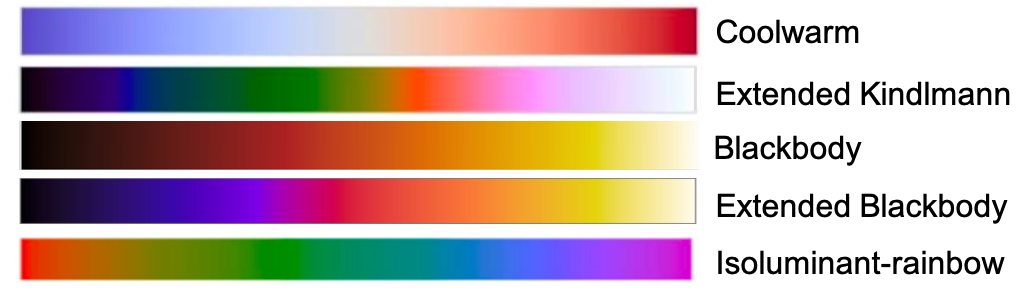
\includegraphics[width = 0.8\columnwidth]{1}
    \caption{ Five Scalar colosmaps. Source:  \cite{???}}
    \label{fig:1}
\end{figure}	

\subsubsection*{Spherical colormappings}
The spherical color mappings are
\begin{itemize}
	\item Absolute value method [cite] is a commonly used color mapping which maps the major axes, to major color components Red, Greed and Blue. The mapping is defined as 
	\begin{equation}
		f(\mathbf{s})=[|s_x|, \ |s_y|, \ |s_z|]^T
	\end{equation}
	where $\mathbf{s}=[s_x ,s_y, s_z]^T$ is the normalized vector corresponding to a line segment.  
	\begin{figure}
		\centering
		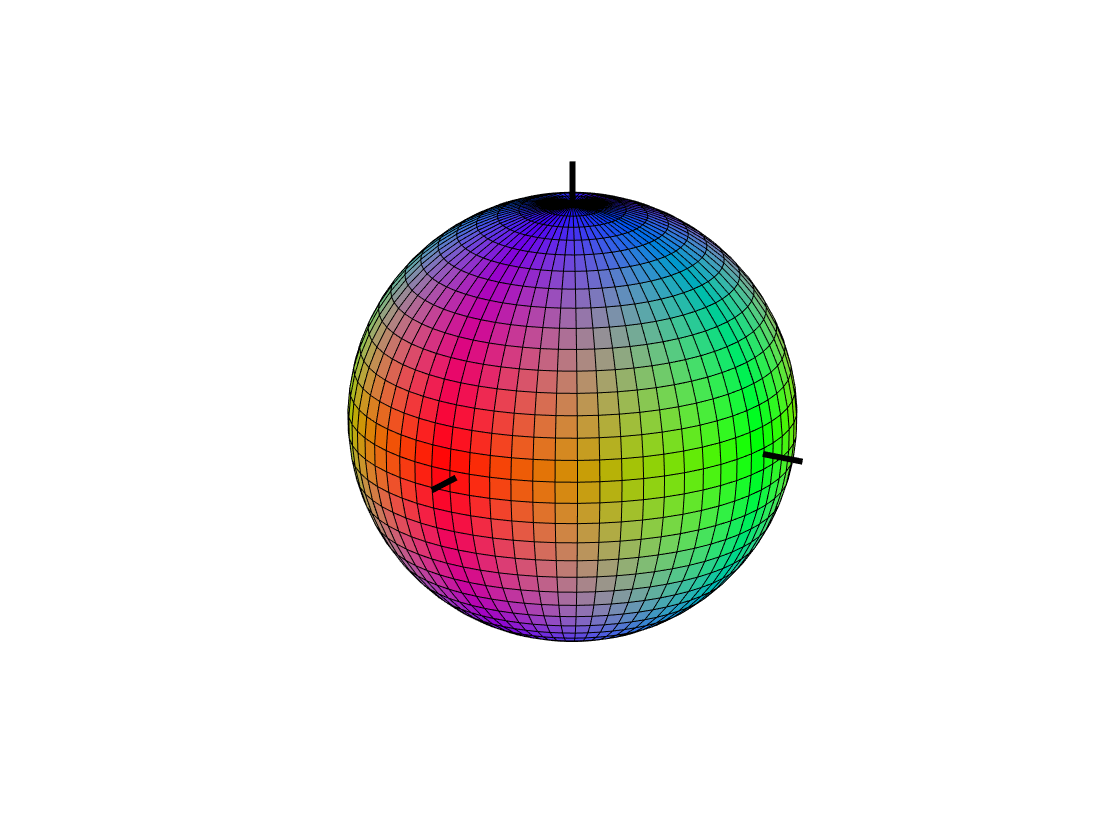
\includegraphics[width=0.35\textwidth]{absolute}
		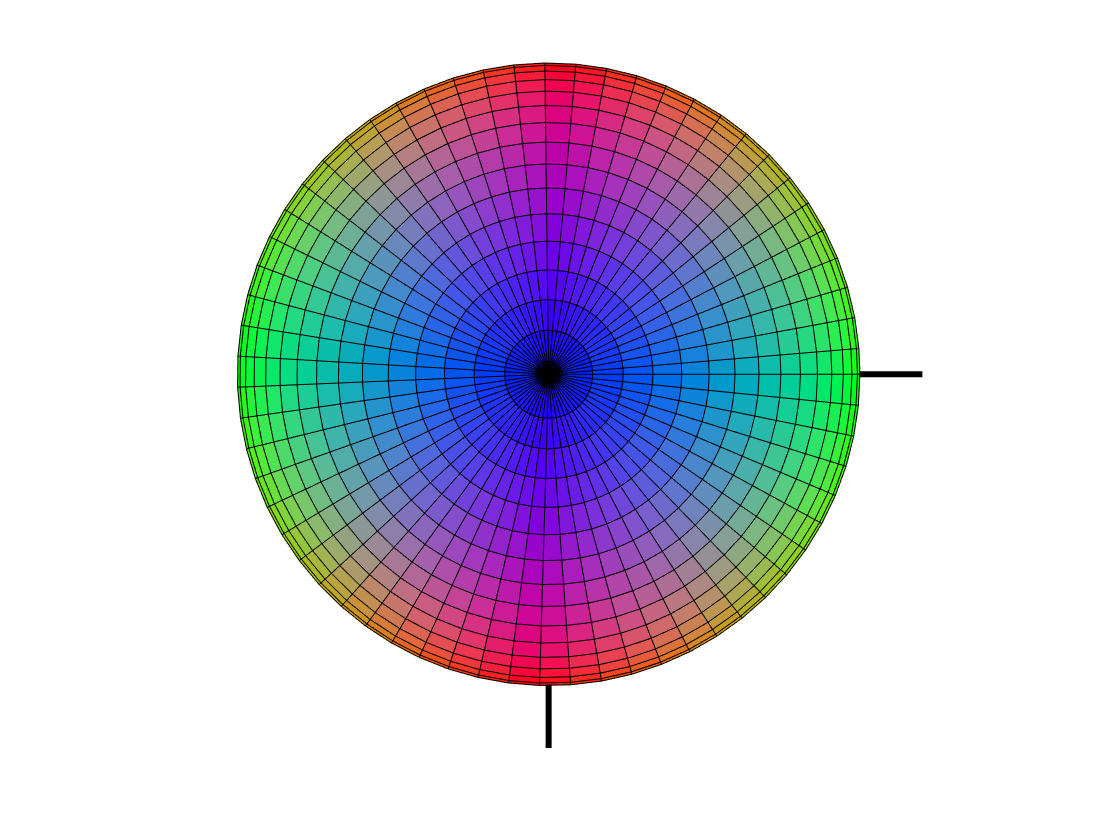
\includegraphics[width=0.3\textwidth]{absolute_top}
		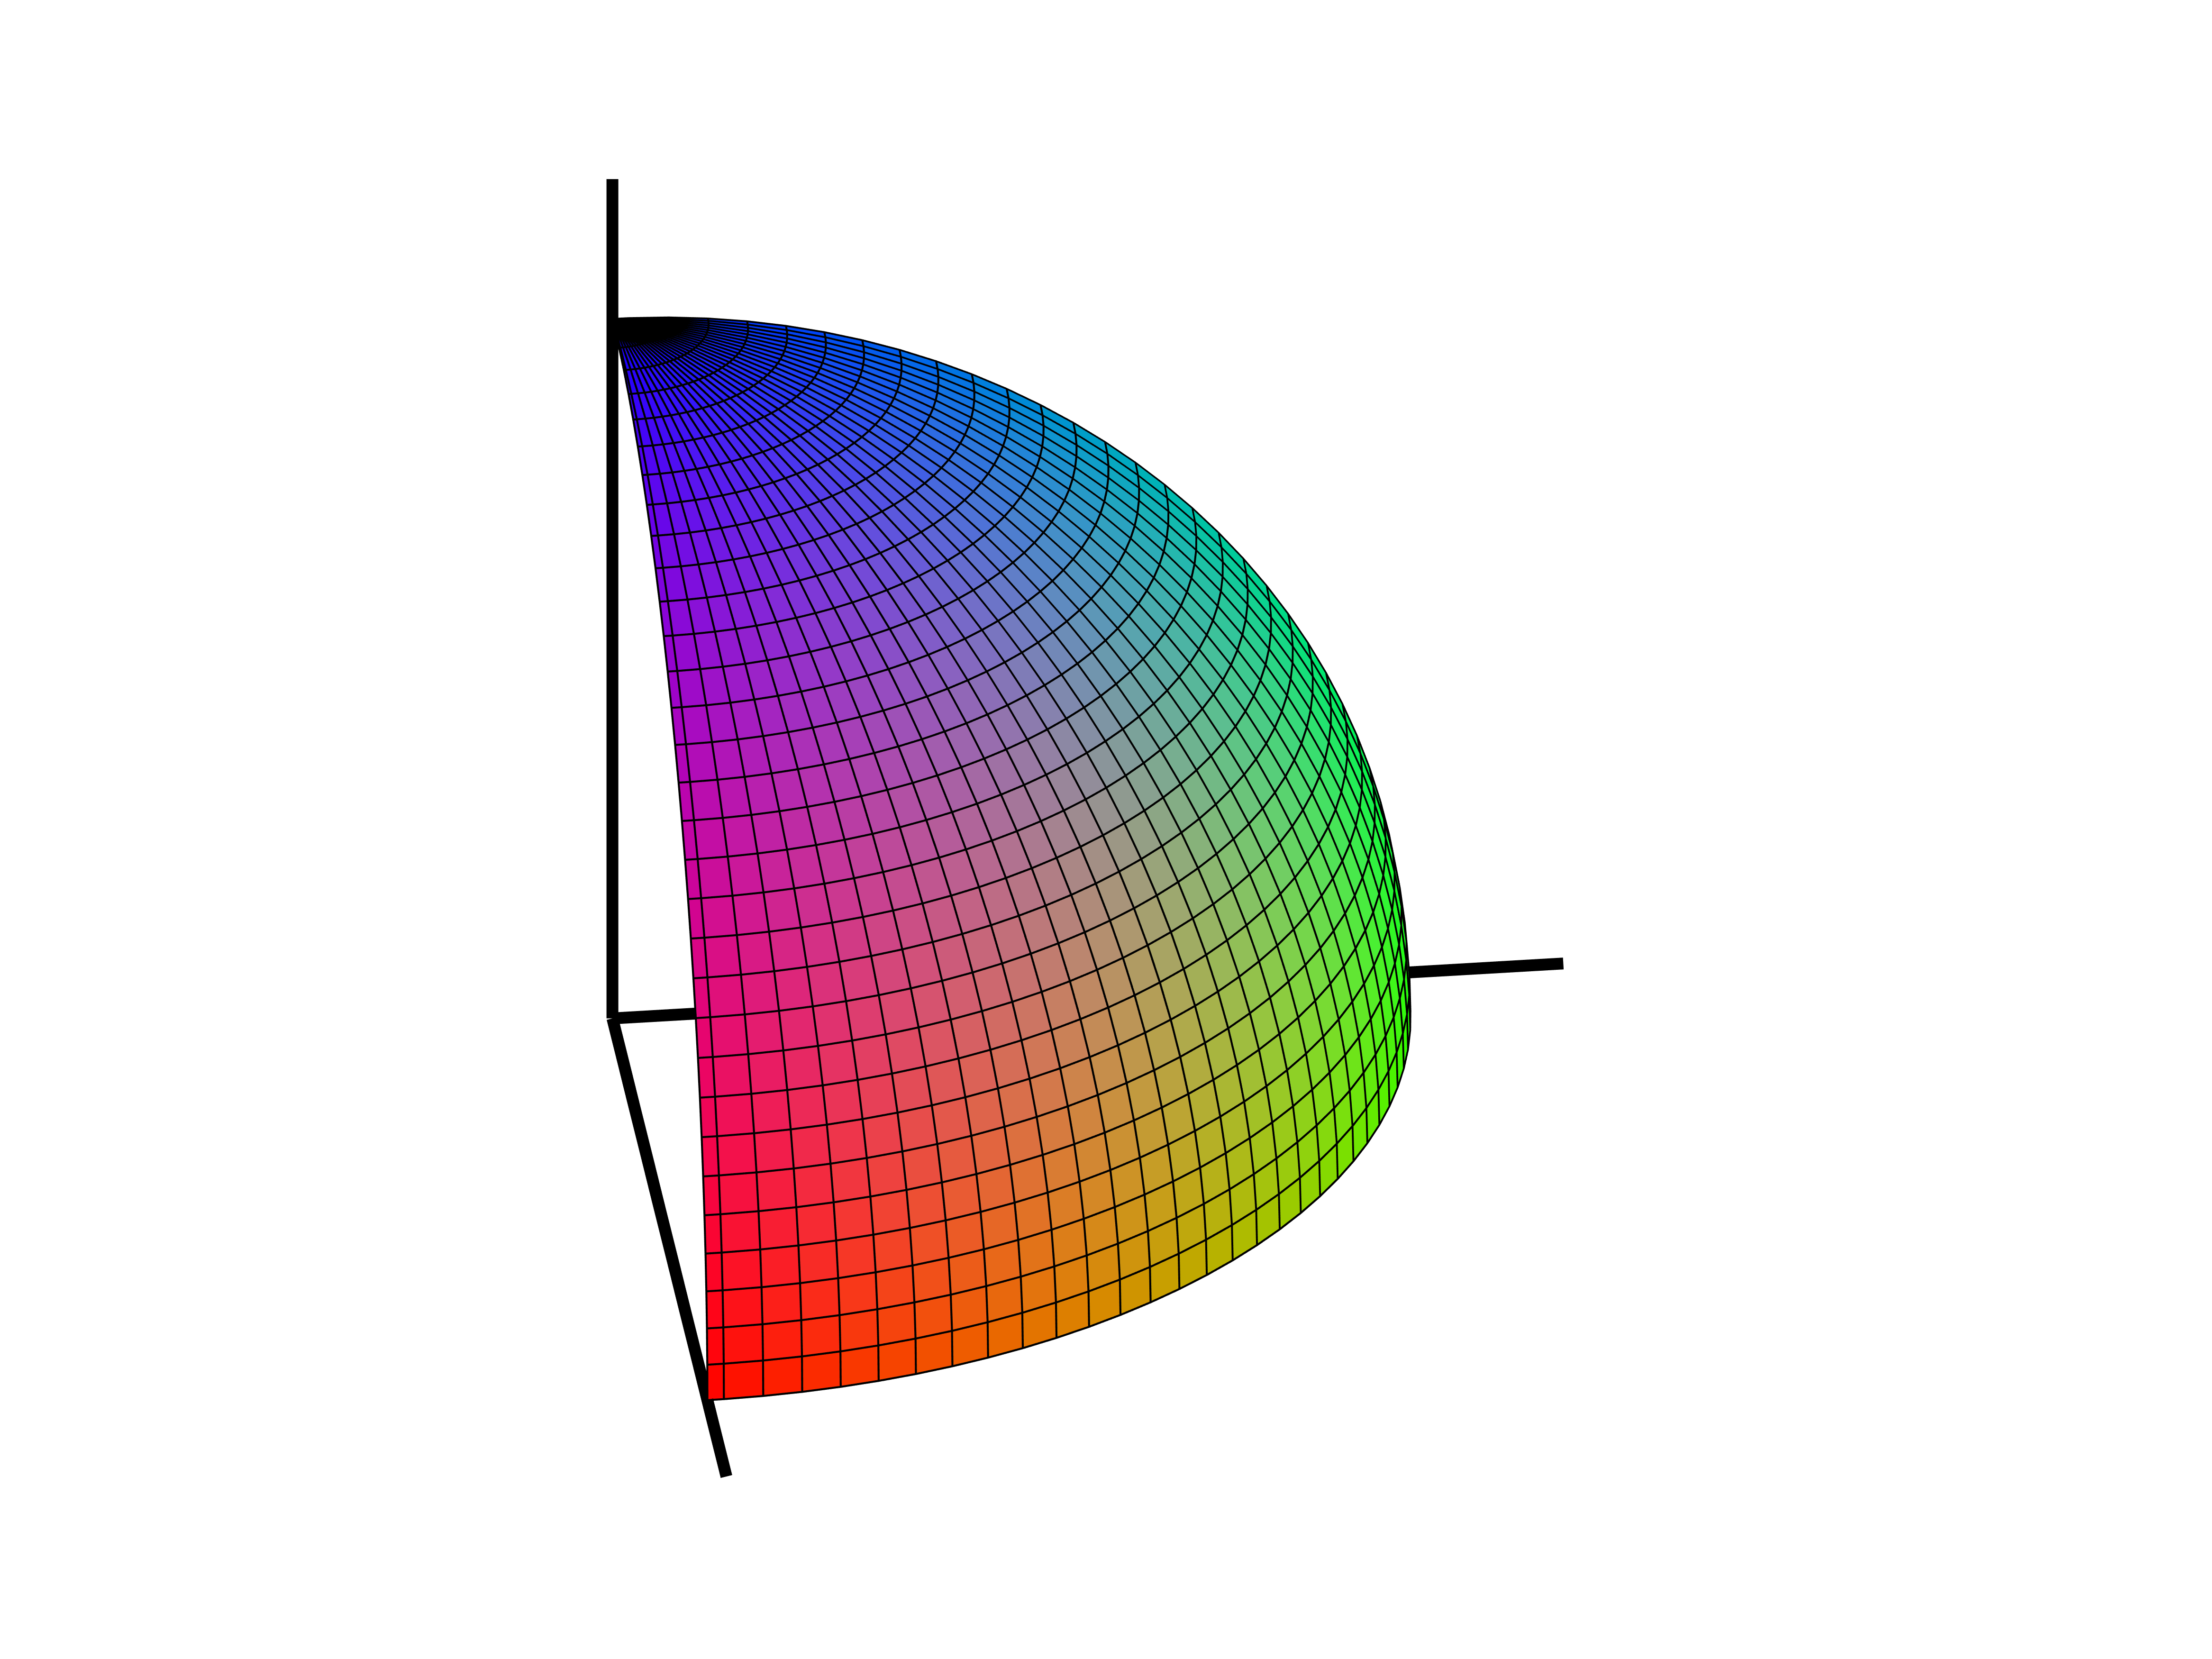
\includegraphics[width=0.3\textwidth]{absolute_octant}
		\caption{Absolute value method, colored sphere.}
	\end{figure}
	
	\item Boy's surface method is a more complicated color mapping scheme based on the immersion of Real Projective Plane in $\mathbb{R}^2$. The mapping is defined as 
	\begin{equation}
		f(\mathbf{s})=[f_1(\mathbf{s}), f_2(\mathbf{s}), f_3(\mathbf{s})]^T
	\end{equation}
	where 
	\begin{equation}
		f_i(\mathbf{s})=\sum_{j=0}^{\infty} c_{i,j} h_j(\mathbf{s}).
	\end{equation}
	
The functions $h_j$ are the spherical harmonics, a similar concept to harmonics in Fourier analysis. As suggested by the authors in [cite], the summation is replaced with a partial sum to obtain a continuous mapping and the coefficients $c_{i,j}$ are adjusted manually for better results. 
\end{itemize}

	\begin{figure}
		\centering
		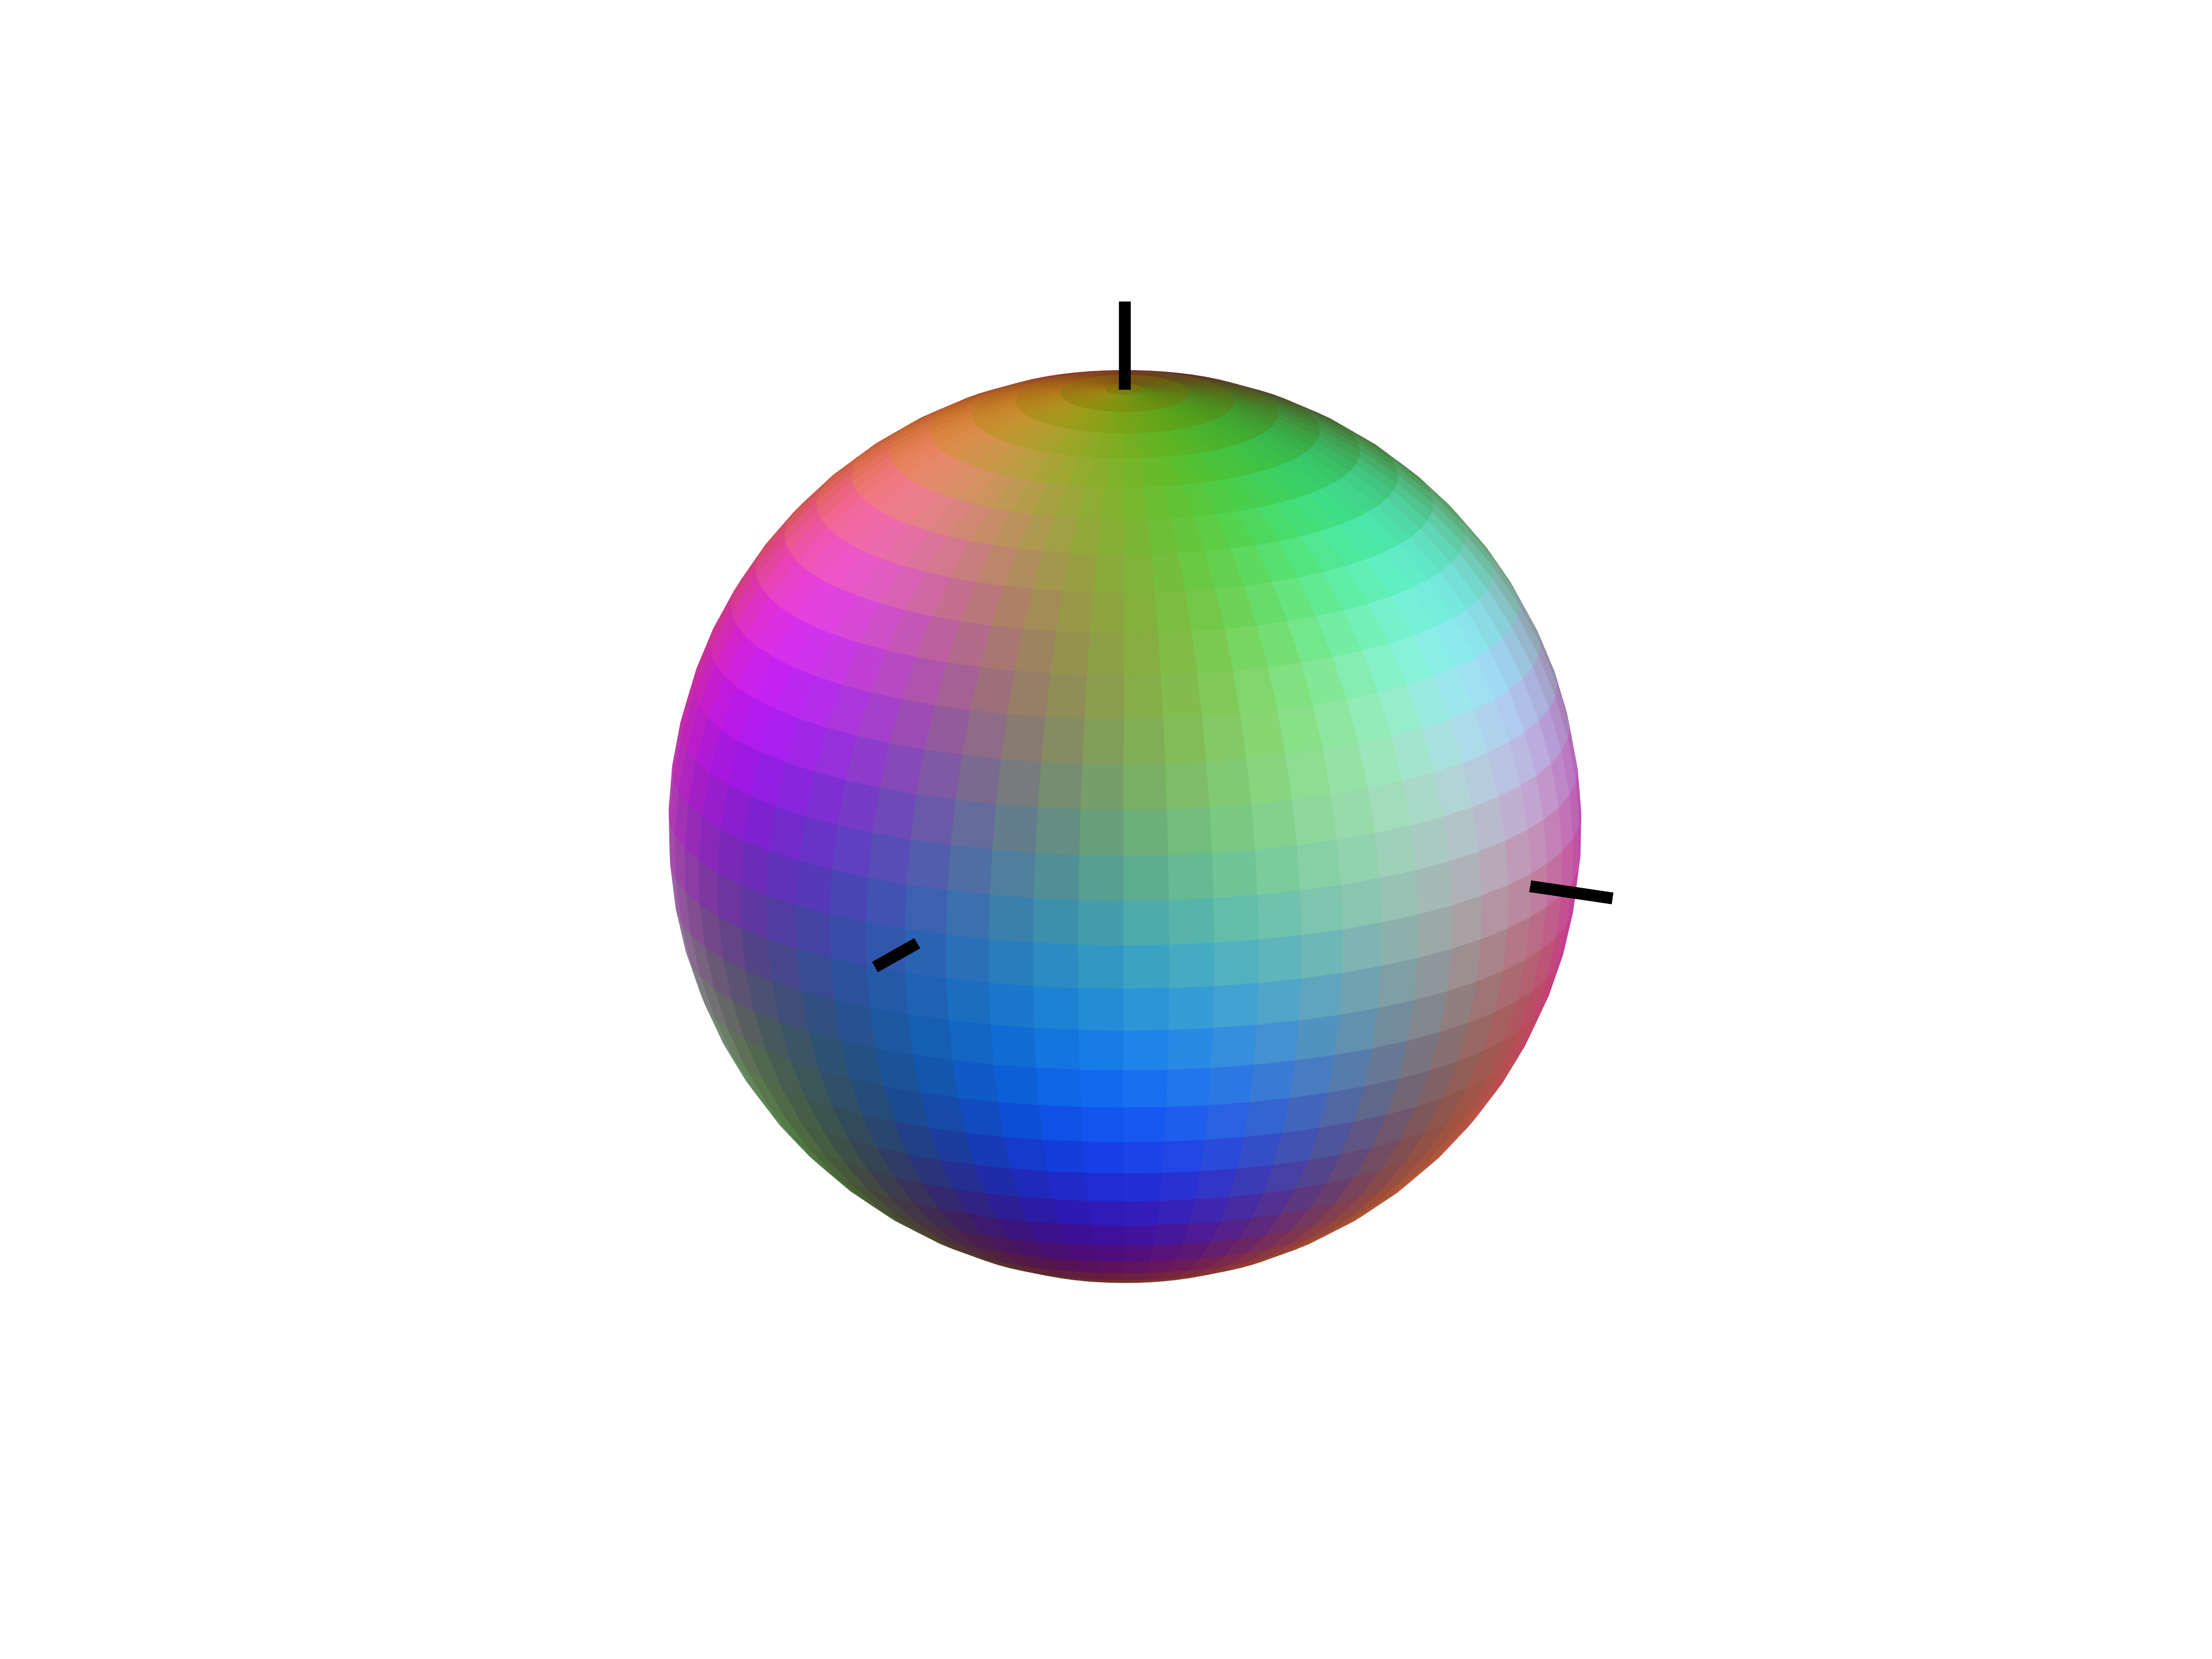
\includegraphics[width=0.33\textwidth]{boys}
		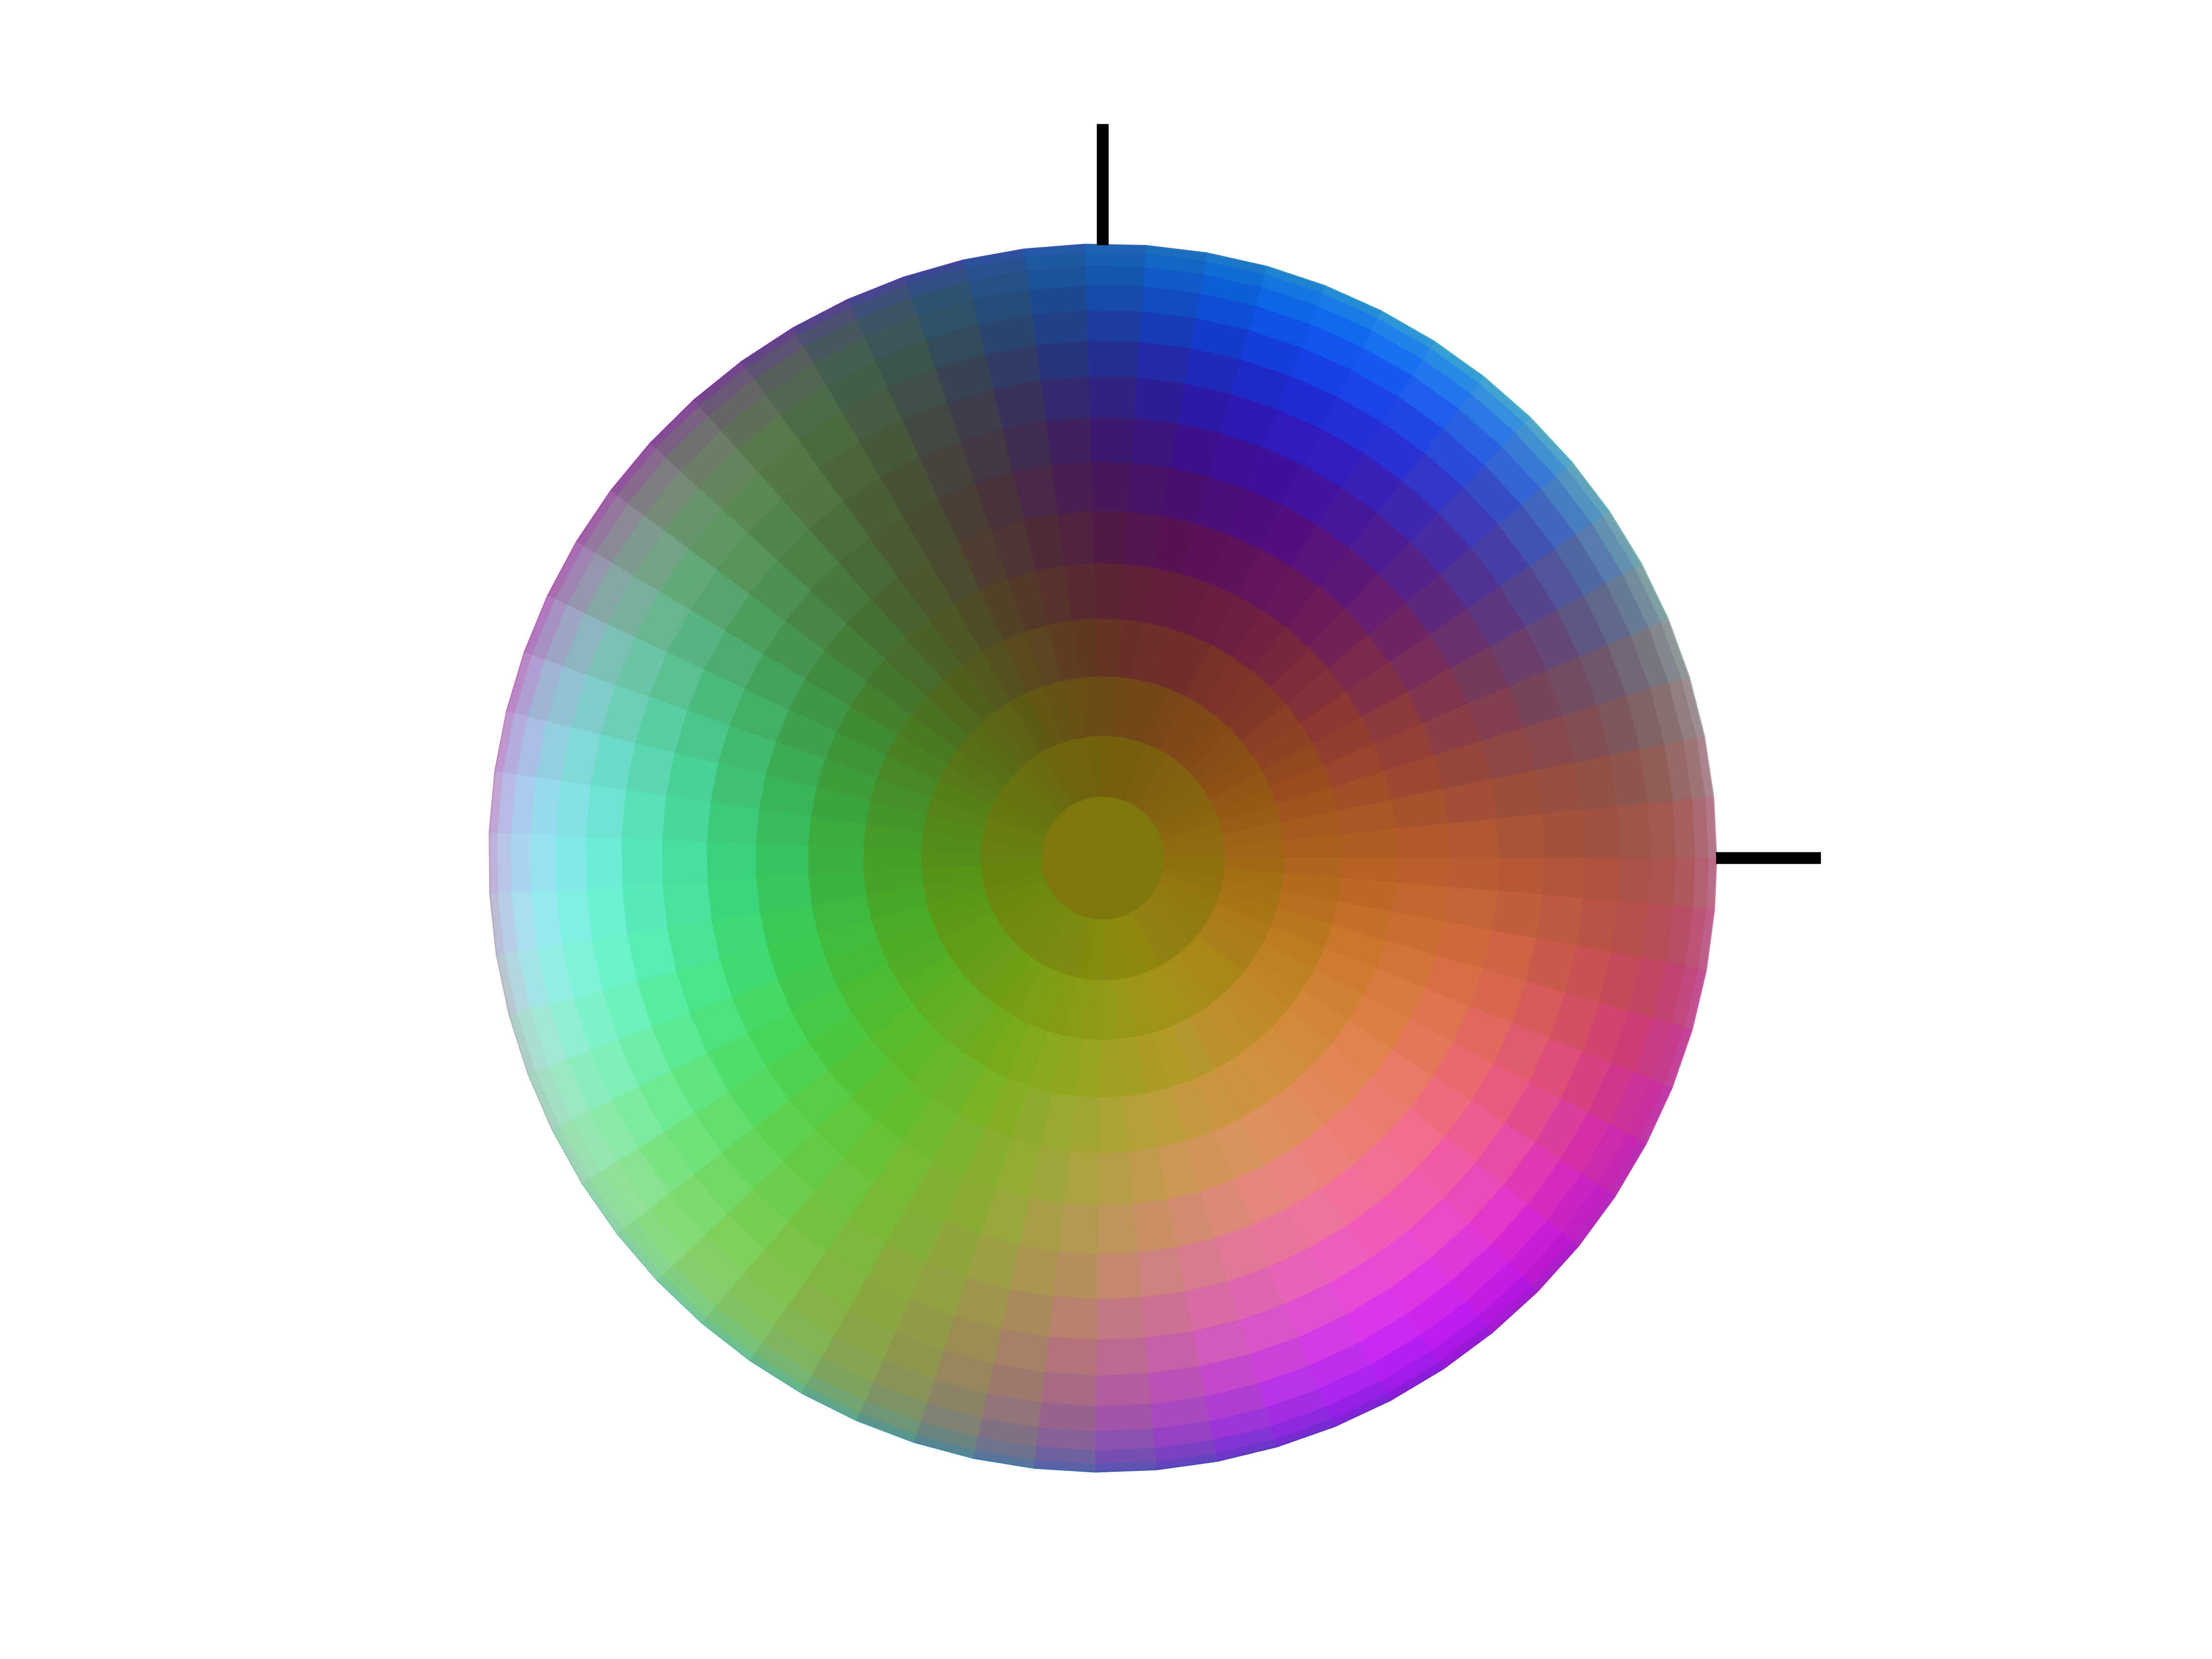
\includegraphics[width=0.3\textwidth]{boys_zIn_yRight}
		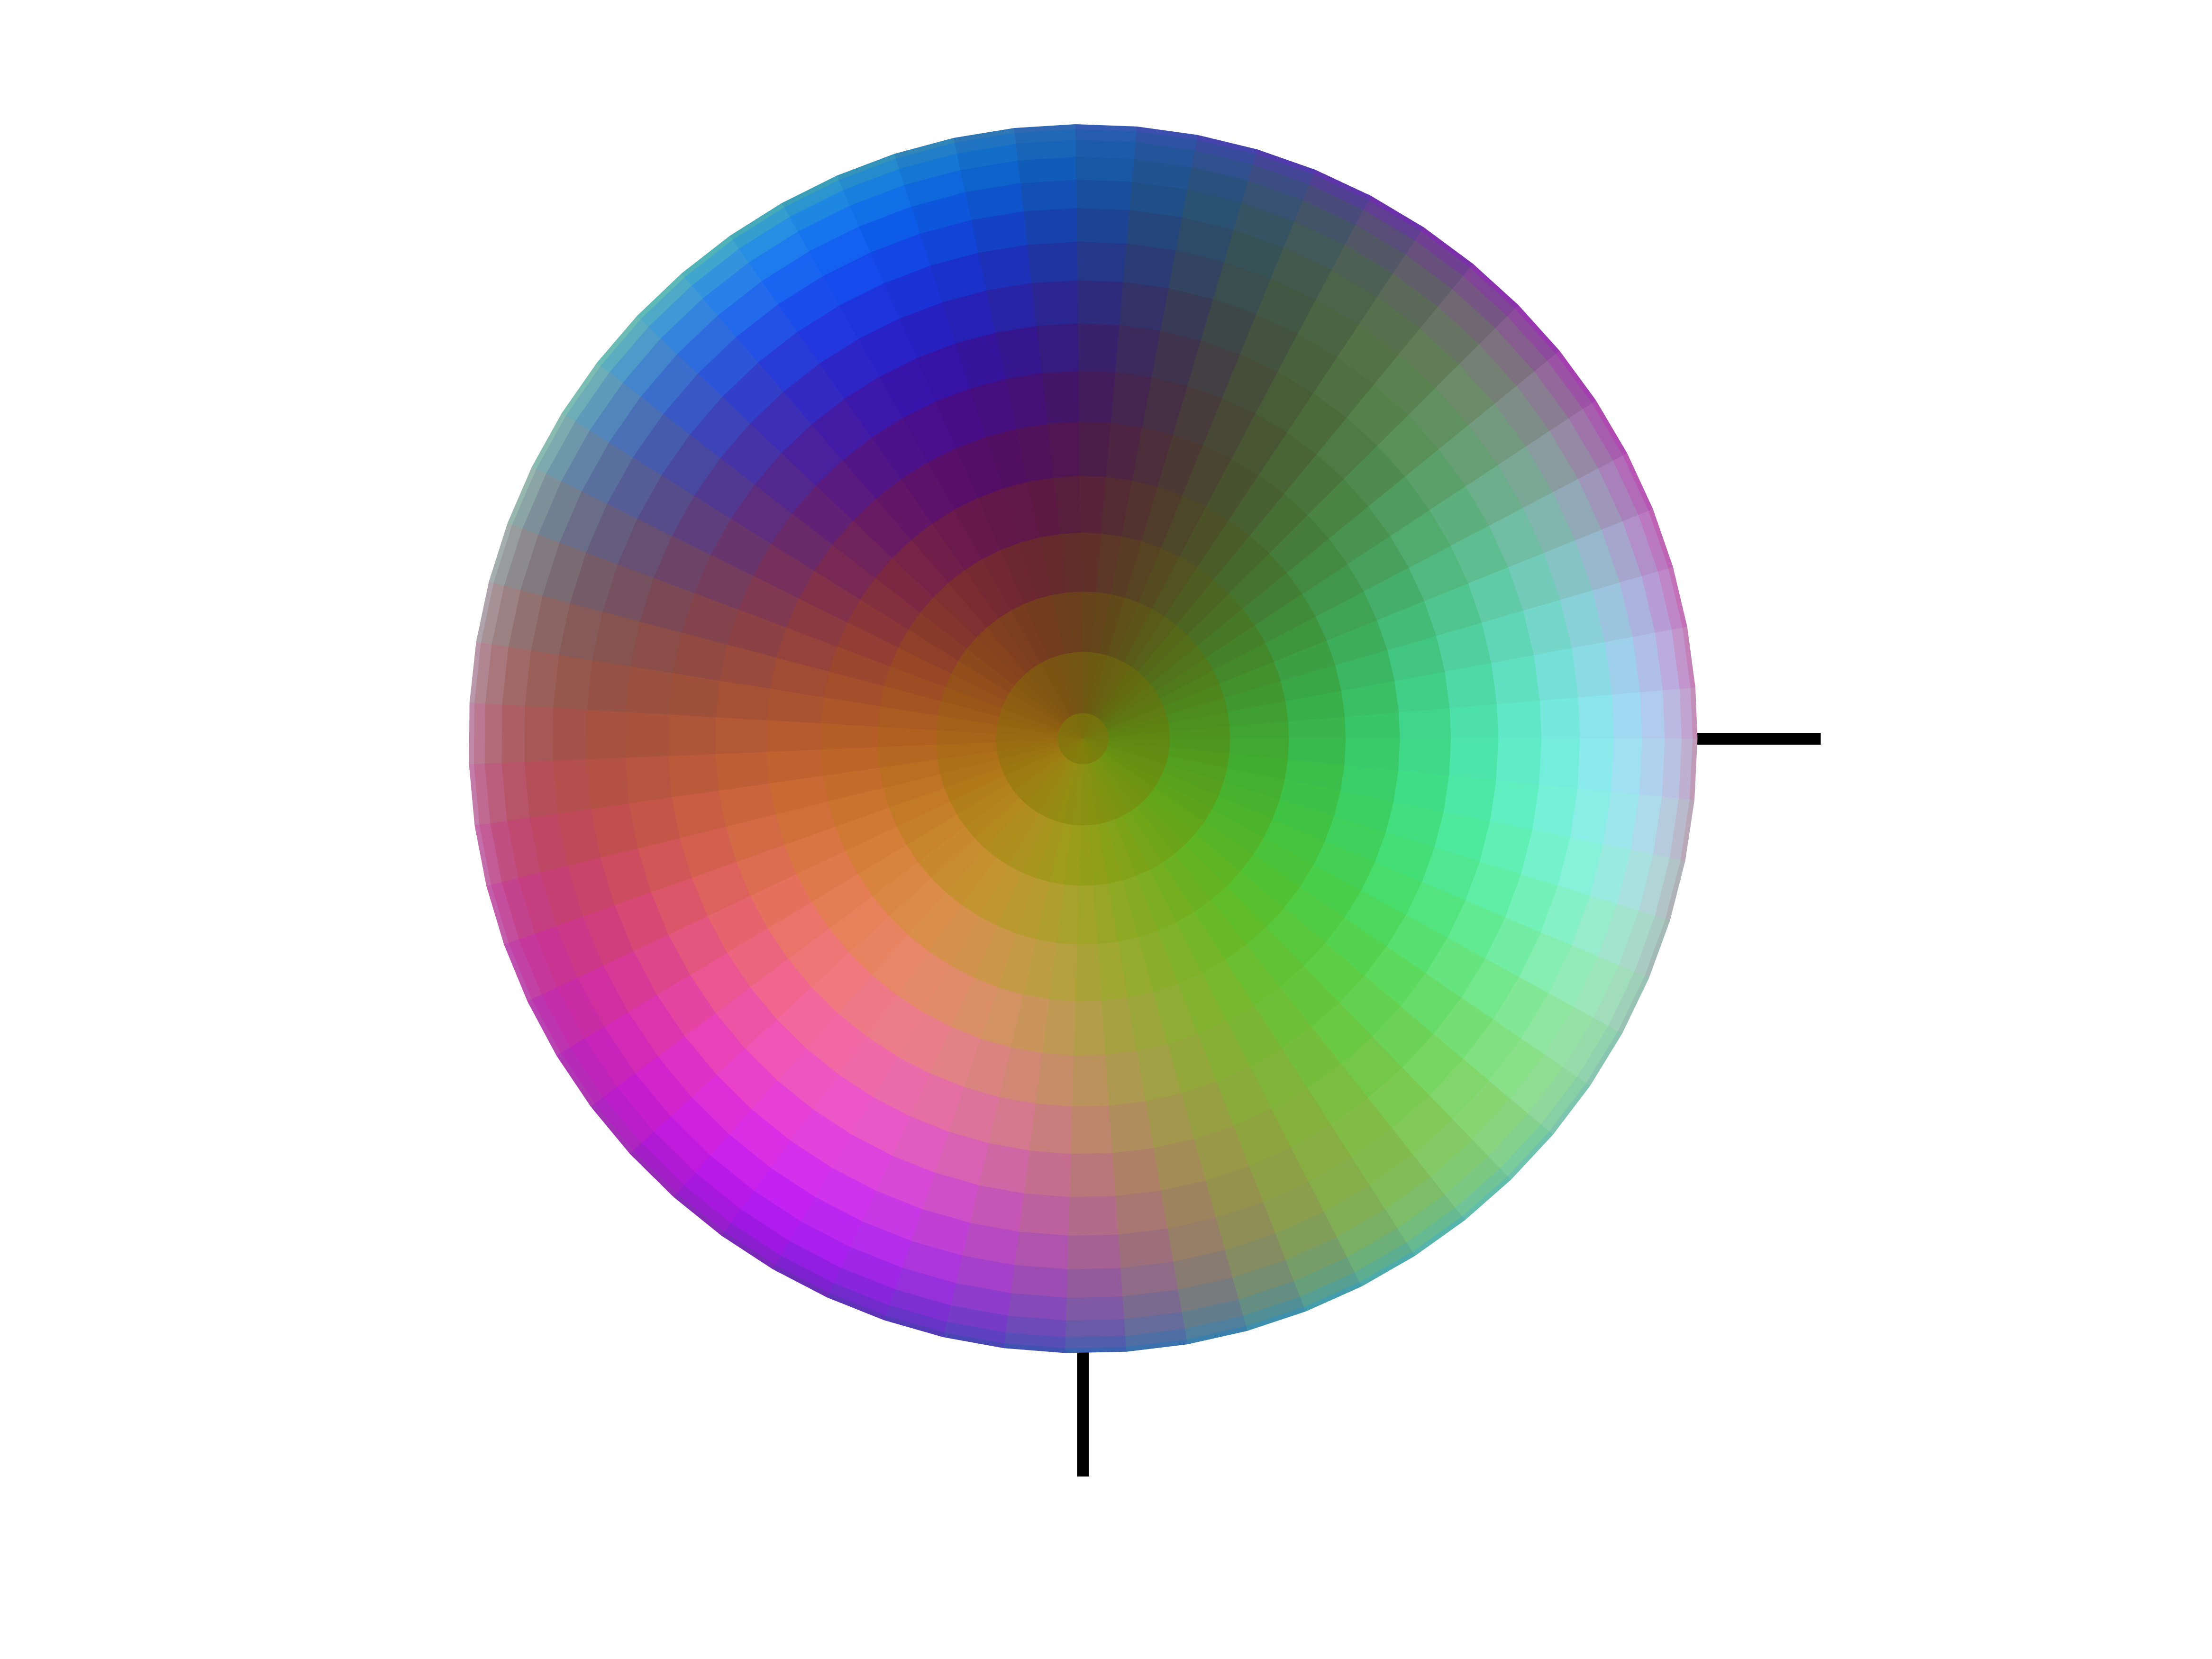
\includegraphics[width=0.3\textwidth]{boys_zOut_yRight}
		\caption{Boy's surface method, colored sphere.}
	\end{figure}

\subsection{Data acquirement}
We converted Digital Imaging and Communications in Medicine (DICOM) file of brain scans, which is presented in 55-slice into Neuroimaging Informatics Technology Initiative (NIFTI) file. Figure~\ref{fig:2} is the presentation of 55 slices of brain scan.

\begin{figure}[ht]
    \centering
    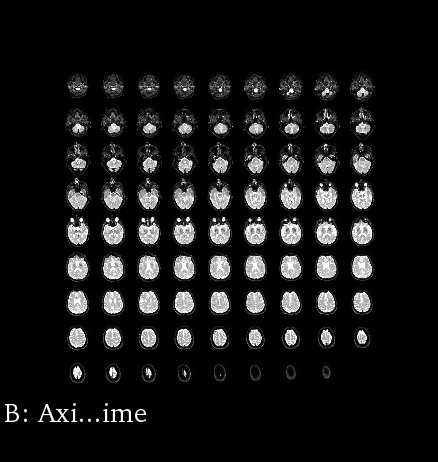
\includegraphics[width = 0.6\columnwidth]{2}
    \caption{ Slice of DICOM  Source:  \cite{???}}
    \label{fig:2}
\end{figure}	

Our first step is brain extraction, using the suitable threshold, which removes non-brain tissue to help with the brain data acquirement. Then we used extracted part to calculate Fractional Anisotropy (FA) and Mean Diffusivity (MD) with the help of FMRIB Software Library (FSL) tool. Finally, we got the Eigenvalues Variance(normalized) and Eigenvalues Mean in the NIFTI files. As Figure~\ref{fig:3} shown, A is the fractional anisotropy value mapping on the green scale; B is the mean diffusivity value mapping on the red scale.
\begin{figure}[ht]
    \centering
    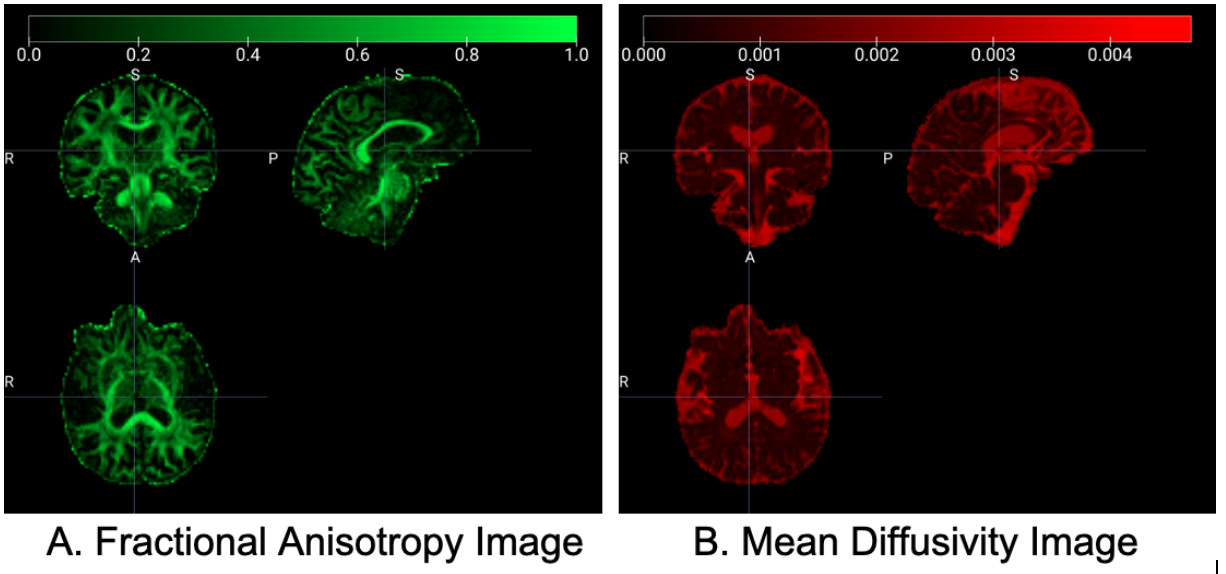
\includegraphics[width = 0.7\columnwidth]{3}
    \caption{ Fractional Anisotropy image and Mean Diffusivity image. Source:  \cite{???}}
    \label{fig:3}
\end{figure}	

\subsection{Rendering}

The brain map read by CGV framework is a TrackVis (trk) file. The data of position is stored in TrackVis file one by one according to the order of the tracts.  Each tract stores two kinds of information, including the offset and the number of points on the current tract, as “Tract (offset, size)”. The Figure~\ref{fig:4} shows the storage mode of TrackVis file. The data read from the NIFTI file with a pointer is in the order of the directory. The storage mode is based on Random Access Storage, i.e., the first dimension to be filled is “x-dimension”, from left to right, then “y-dimension” from posterior to anterior, then “z-dimension”, from inferior to superior. We got the brain data as (116, 116, 80, 55). The first three dimensions are the size of the full volume data in the xyz direction, and the fourth dimension is assumed to refer to time, which also represents the number of slices. The calculated FA and MD data are both with (116, 116, 80, 1). The stored data type is float. The number of voxels is 1,076,480.

\begin{figure}[ht]
    \centering
    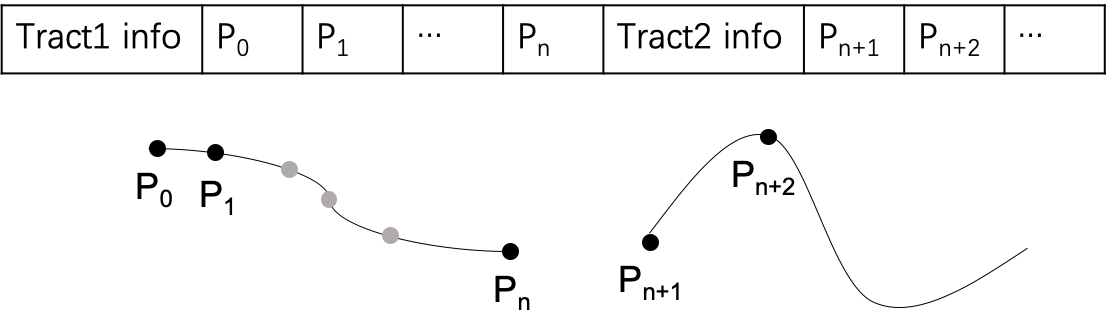
\includegraphics[width = 0.8\columnwidth]{4}
    \caption{Storage mode of TrackVis file. Source:  \cite{???}}
    \label{fig:4}
\end{figure}	

In order to access a one-to-one correspondence between the FA/MD data and the brain tract positions, we calculated the bounding box of FA/MD data, which is to eliminate the voxels whose FA and MD values are 0. After that we ordered the eliminated data again and stored them in a new vector. The dimension of the processed data is (70, 82, 76, 1) on xyzt dimension. The number of voxels is 436,240. (Figure~\ref{fig:5})

\begin{figure}[ht]
    \centering
    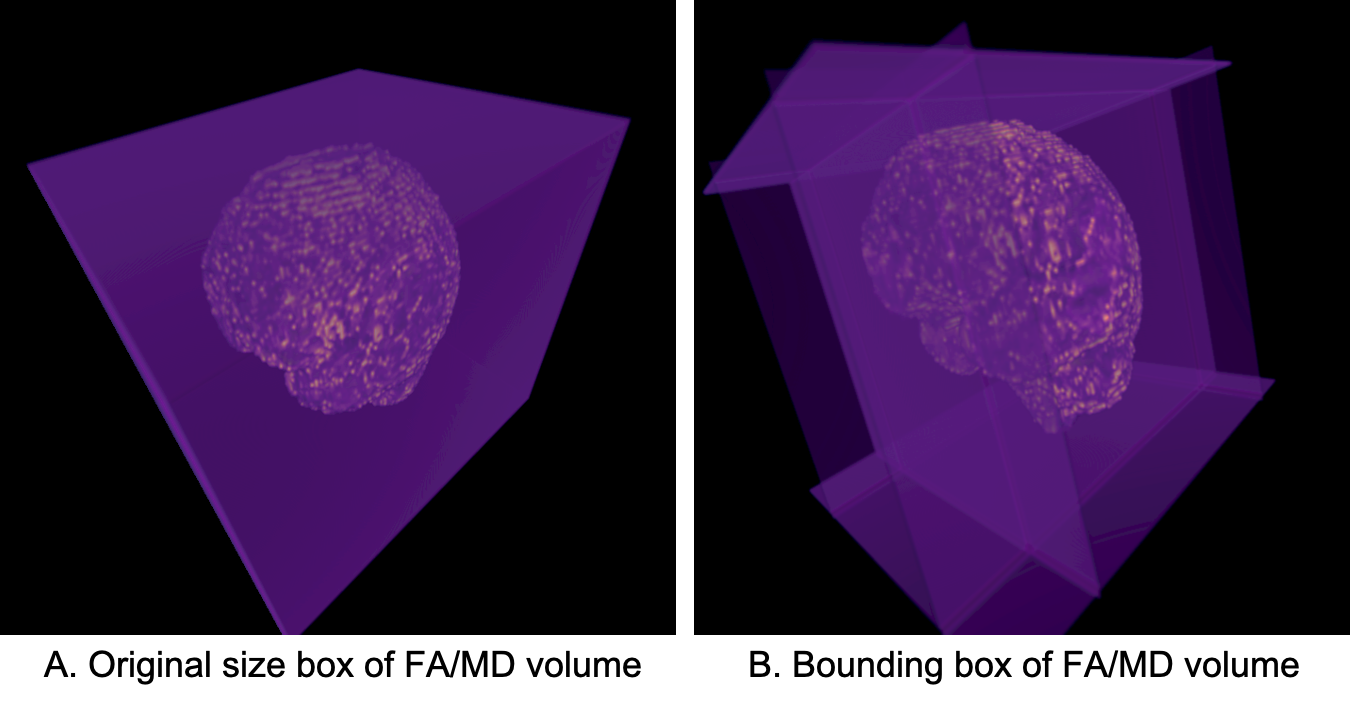
\includegraphics[width = 0.8\columnwidth]{5}
    \caption{Sketch of size cutting. Source:  \cite{???}}
    \label{fig:5}
\end{figure}	

Since the dimensional order of data rendering in Opengl is in xzy-oder, and the storage order of FA/MD data are in xyz-order, we have transformed the data through the corresponding between coordinate and index. As it shown in Figure~\ref{fig:6}, we mapped the FA/MD value on tractography volume with size matching and dimension swapping.

\begin{figure}[ht]
    \centering
    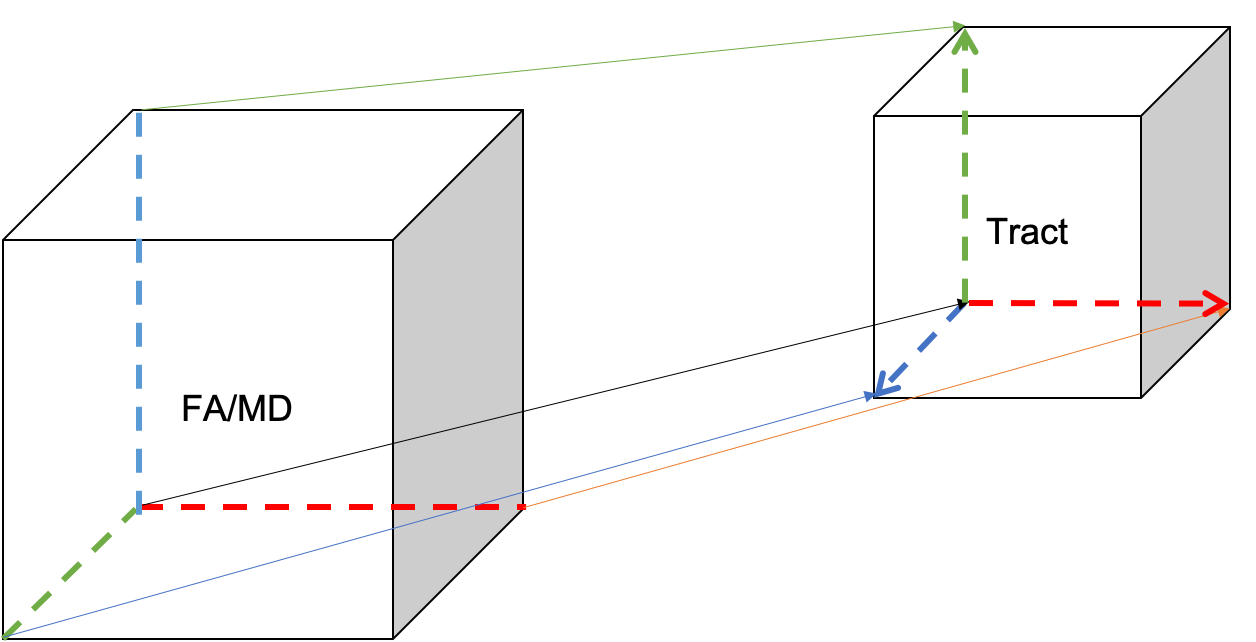
\includegraphics[width = 0.8\columnwidth]{6}
    \caption{Sketch of size matching and dimension swapping between FA/MD and Tractography. Source:  \cite{???}}
    \label{fig:6}
\end{figure}	

After mapping FA and MD to different color map values and mapping them to the corresponding tract positions, we get ten different brain maps. As it shown in the Figure~\ref{fig:7} and \ref{fig:8}.

\begin{figure}[ht]
    \centering
    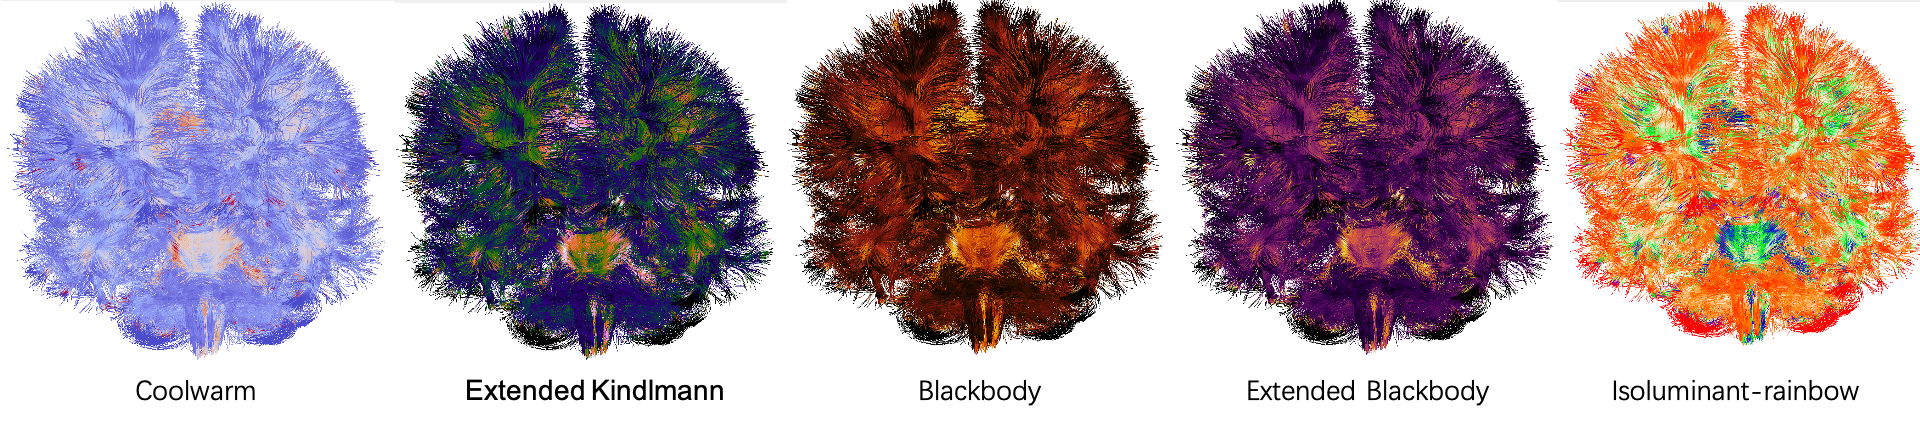
\includegraphics[width = 0.9\columnwidth]{7}
    \caption{Tractography of FA in different colormap. Source:  \cite{???}}
    \label{fig:7}
\end{figure}

\begin{figure}[ht]
    \centering
    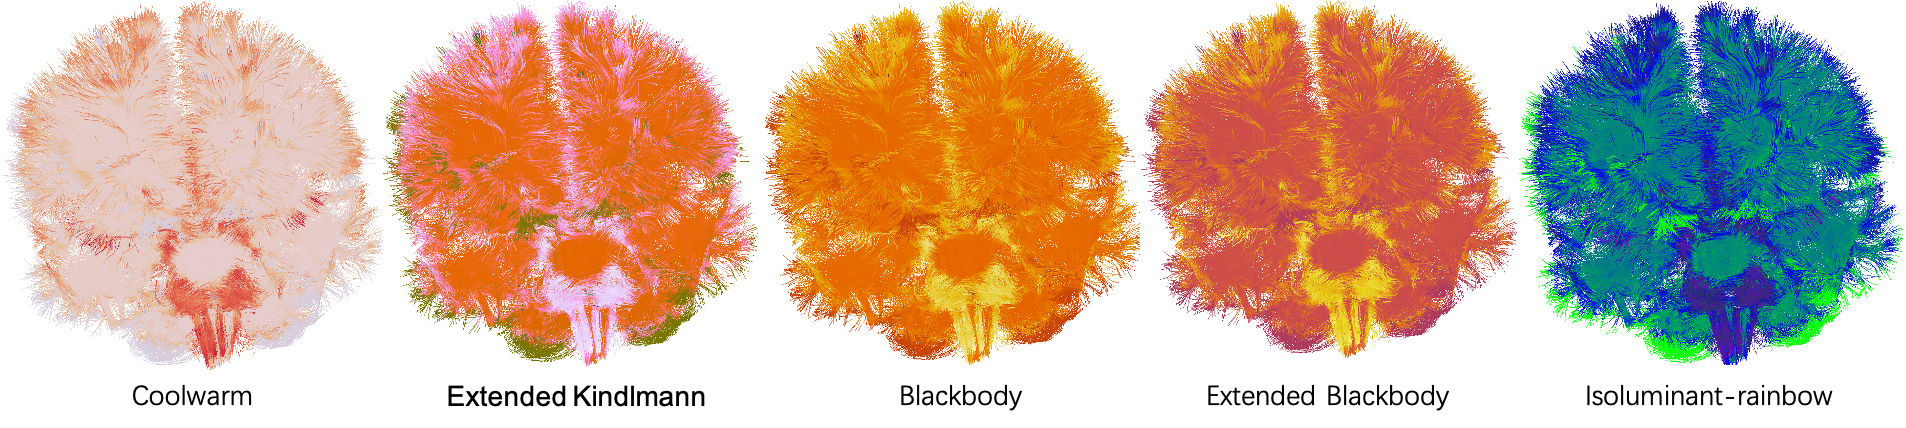
\includegraphics[width = 0.9\columnwidth]{8}
    \caption{Tractography of MD in different colormap. Source:  \cite{???}}
    \label{fig:8}
\end{figure}

\section{Evaluation}

\subsection{Participants }
In our study, we selected 15 participants ( ...male and ... female) of mean age .... with standard deviation ..... 
The program ran on a ..........Their majors were: ....in ..., ....in ....,.  All participants have normal vision. 

\subsection{Enviornment}
The room had natural light and the display was a ......... The stereo rendering was ........
Participants sat on a normal chair.

\subsection{Procedure}
All participants first tested for normal vision with the Ishihara Color vision test. This test is online and is well-known as the Color Blind test and it is the most widely used color vision test all around the world. There are some numbers surrounded with dots and the user should distinguish the numbers out of the dots (Figure~\ref{fig: Ishihara}). If the person can get the normal color vision score it means that the user can see up to one million distinct shades of color.
\begin{figure}[ht]
    \centering
    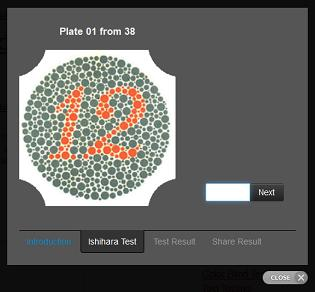
\includegraphics[width = 0.6\columnwidth]{Ishihara}
    \caption{Ishihara color blindness test. Source:  \cite{www.color-blindness.com}}
    \label{fig:Ishihara}
\end{figure}

For understanding the tasks each participants received general information about the test structure, DMRI techniques and their medical applications. These information took about 10 minutes. 

All participants were told to finish the test as soon as possible. But they could take a break at anytime. The questionnaire time was started when the user started the test until the final task was answered. 
All of them examined all colormaps.


\end{document}
